	% Szglab4
% ===========================================================================
%
\chapter{Analízis modell kidolgozása 2}

\thispagestyle{fancy}

\section{Objektum katalógus}

\comment{Minden, a feladatban szereplő objektum rövid, egy-két bekezdés hosszú ismertetése. Meg kell jelenjen minden objektumhoz, hogy mi a felelőssége. Informális leírás, ezért nem kell foglalkozni az örökléssel, az interfészekkel, az absztrakt osztályokkal, a segédosztályokkal.}

\subsection{Objektum1}
\comment{Felelősség informális leírása}

\subsection{Objektum2}
\comment{Felelősség informális leírása}

\section{Statikus struktúra diagramok}
\comment{Az előző alfejezet osztályainak kapcsolatait és publikus metódusait bemutató osztálydiagram(ok). Tipikus hibalehetőségek: csillag-topológia, szigetek.}

\begin{figure}[h]
\begin{center}
%\includegraphics[width=17cm]{chapters/chapter04/example.pdf}
\caption{x}
\label{fig:example3}
\end{center}
\end{figure}


\section{Osztályok leírása}
\comment{Az előző alfejezetben tárgyalt objektumok felelősségének formalizálása attribútumokká, metódusokká. Csak publikus metódusok szerepelhetnek. Ebben az alfejezetben megjelennek az interfészek, az öröklés, az absztrakt osztályok. Segédosztályokra még mindig nincs szükség. Az osztályok ABC sorrendben kövessék egymást. Interfészek esetén az Interfészek, Attribútumok pontok kimaradnak.}

\subsection{Osztály1}
\begin{itemize}
\item Felelősség\\
\comment{Mi az osztály felelőssége. Kb 1 bekezdés.}
\item Ősosztályok\\
\comment{Mely osztályokból származik (öröklési hierarchia)\newline
Legősebb osztály $\rightarrow$ Ősosztály2 $\rightarrow$ Ősosztály3...}
\item Interfészek\\
\comment{Mely interfészeket valósítja meg.}
\item Attribútumok\\
\comment{Milyen attribútumai vannak}
	\begin{itemize}
		\item attribútum1: attribútum jellemzése: mire való
		\item attribútum2: attribútum jellemzése: mire való
	\end{itemize}
\item Metódusok\\
\comment{Milyen publikus metódusokkal rendelkezik. Metódusonként egy-három mondat arról, hogy a metódus mit csinál.}
	\begin{itemize}
		\item int foo(Osztály3 o1, Osztály4 o2): metódus leírása
		\item int bar(Osztály5 o1): metódus leírása
	\end{itemize}
\end{itemize}

\subsection{Osztály2}
\begin{itemize}
\item Felelősség\\
\comment{Mi az osztály felelőssége. Kb 1 bekezdés.}
\item Ősosztályok\\
\comment{Mely osztályokból származik (öröklési hierarchia)\newline
Legősebb osztály $\rightarrow$ Ősosztály2 $\rightarrow$ Ősosztály3...}
\item Interfészek\\
\comment{Mely interfészeket valósítja meg.}
\item Attribútumok\\
\comment{Milyen attribútumai vannak}
	\begin{itemize}
		\item attribútum1: attribútum jellemzése: mire való
		\item attribútum2: attribútum jellemzése: mire való
	\end{itemize}
\item Metódusok\\
\comment{Milyen publikus metódusokkal rendelkezik. Metódusonként egy-három mondat arról, hogy a metódus mit csinál.}
	\begin{itemize}
		\item int foo(Osztály3 o1, Osztály4 o2): metódus leírása
		\item int bar(Osztály5 o1): metódus leírása
	\end{itemize}
\end{itemize}

\section{Szekvencia diagramok}
\comment{Inicializálásra, use-case-ekre, belső működésre. Konzisztens kell legyen az előző alfejezettel. Minden metódus, ami ott szerepel, fel kell tűnjön valamelyik szekvenciában. Minden metódusnak, ami szekvenciában szerepel, szereplnie kell a valamelyik osztálydiagramon.}

\begin{figure}[!htbp]
	\begin{center}
		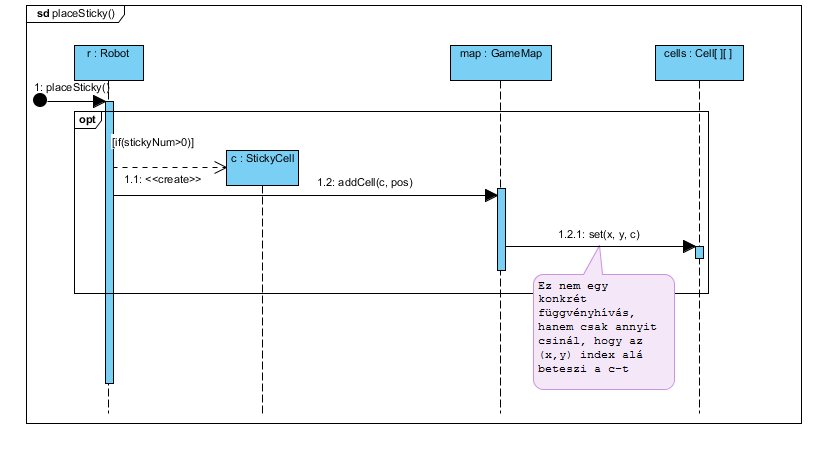
\includegraphics[width=178mm, center]{./chapters/chapter04/sticky.png}
		\caption{Ragacs hátrahagyása}
	\end{center}
\end{figure}

\begin{figure}[!htbp]
	\begin{center}
		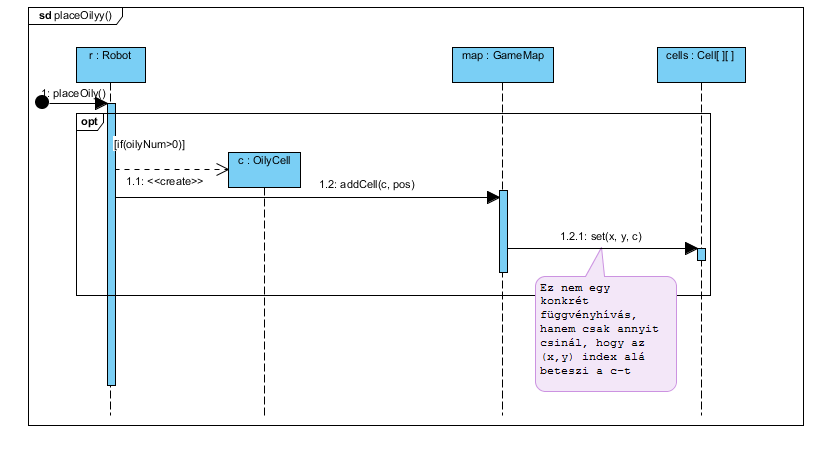
\includegraphics[width=178mm, center]{./chapters/chapter04/oily.png}
		\caption{Olaj hátrahagyása}
	\end{center}
\end{figure}

\begin{figure}[!htbp]
	\begin{center}
		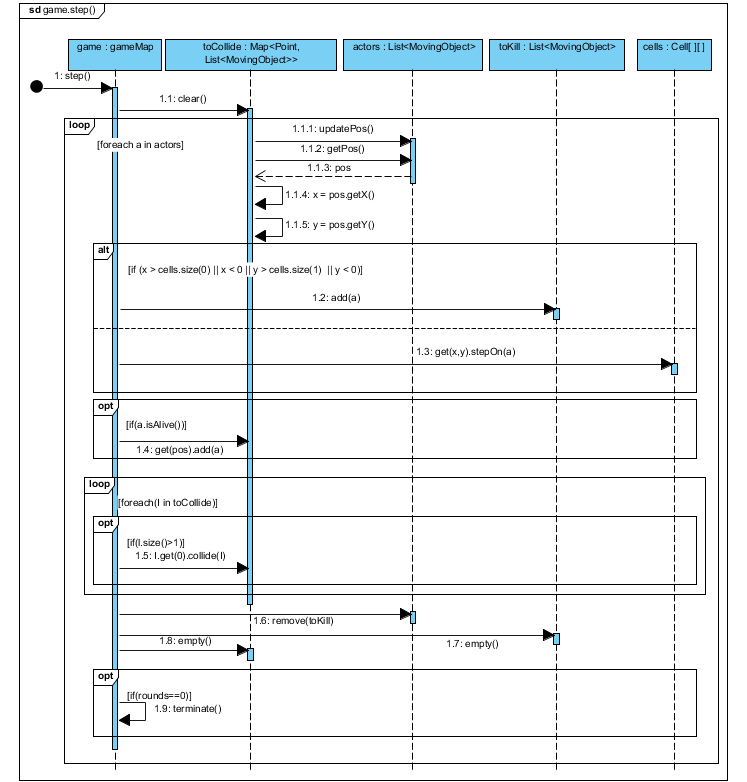
\includegraphics[width=195mm, center]{./chapters/chapter04/step.png}
		\caption{A játék léptetése}
	\end{center}
\end{figure}

\section{State-chartok}
\comment{Csak azokhoz az osztályokhoz, ahol van értelme. Egyetlen állapotból álló state-chartok ne szerepeljenek. A játék működését bemutató state-chart-ot készíteni tilos.}

\begin{figure}[h]
\begin{center}
%\includegraphics[width=17cm]{chapters/chapter04/example.pdf}
\caption{x}
\label{fig:example3}
\end{center}
\end{figure}

